\begin{enumerate}
	\item \textbf{Deactivate Voter}
		\begin{enumerate}
			\item \textbf{Service Contract}
				\begin{figure}[H]
					\centering
					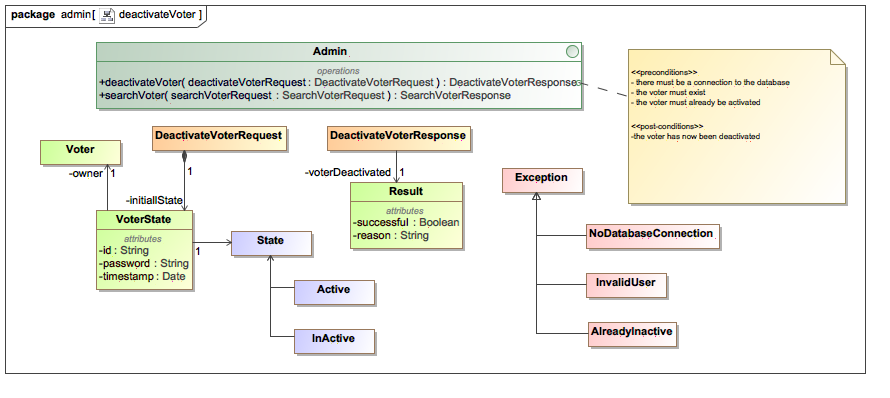
\includegraphics[width=0.75\linewidth]{../Images/Admin/ServiceContracts/deactivateVoter_ServiceContract.png}
					\caption{Deactivate Voter Service Contract}
				\end{figure}
				
				Deactivate Voter requires an ID number in the request which will be used to change the ActiveState state to inactive if all pre-conditions are met.
				\newline	
								
				\begin{enumerate}
					\item Pre-conditions
					\begin{itemize}
						\item There must be a connection to the database
						\item The voter must exist
						\item the voter must already be activated
					\end{itemize}
					
					\item Exceptions
					\begin{itemize}
						\item If there is no connection to the database, the NoDatabaseConnection exception will be thrown
						\item If a voter's ID is not valid, the IdDoesNotExist exception will be thrown
						\item If the voter is already active, the AlreadyActive exception will be thrown
					\end{itemize}
					
					\item Post-conditions
					\begin{itemize}
						\item The voter is now deactivated
					\end{itemize}
				\end{enumerate}
			
			\newpage
			
			\item \textbf{Functional Requirements}
				\begin{figure}[H]
					\centering
					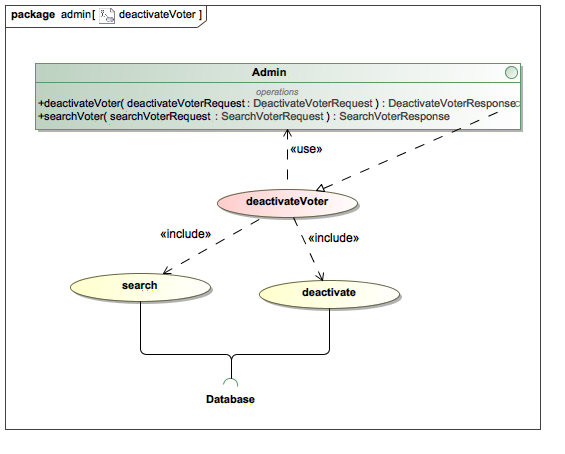
\includegraphics[width=0.75\linewidth]{../Images/Admin/UseCases/deactivateVoter_useCase.png}
					\caption{Deactivate Voter Use Case}
				\end{figure}
				
				The Deactivate Voter process will call the DeactivateVoter use case from the database module.
				\newline
				
			\item \textbf{Process Design}
				\begin{figure}[H]
					\centering
					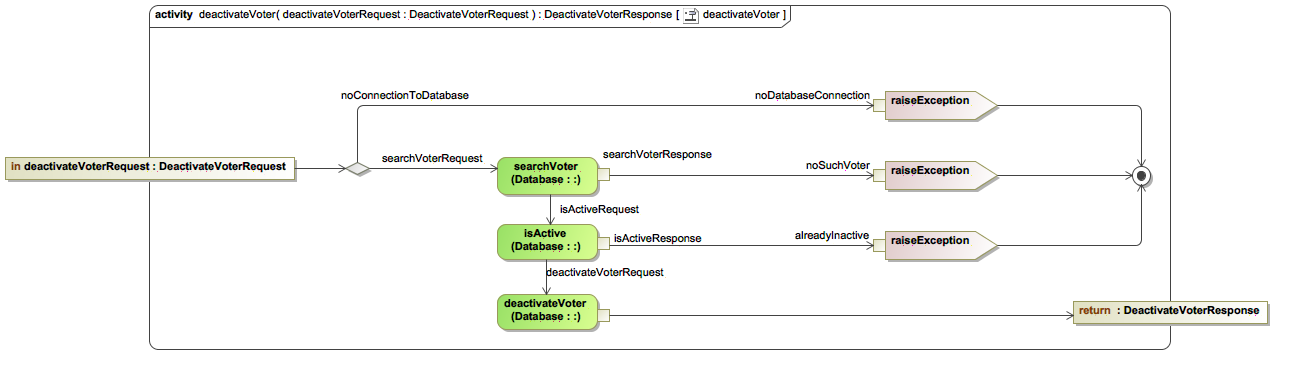
\includegraphics[width=0.75\linewidth]{../Images/Admin/ActivityDiagrams/deactivateVoter_ActivityDiagram.png}
					\caption{Deactivate Voter Activity}
				\end{figure}
				
				The Deactivate Voter process will first retrieve the ID number from the request and validate if is a valid ID number, after which it will get all the necessary Voter details from the database which corresponds to that ID number. It then checks in what state the voter is to see if it has already been deactivated. If all cases are valid, then the voter's ActiveState will change from Valid to Invalid.
				\newline
				
		\end{enumerate}
		
		\newpage
		
		\item \textbf{Add Party}
		\begin{enumerate}
			\item \textbf{Service Contract}
			\begin{figure}[H]
				\centering
				\includegraphics[width=0.75\linewidth]{../Images/Admin/ServiceContracts/addParty_ServiceContract.png}
				\caption{Add Party Service Contract}
			\end{figure}
			
		Adding a new political party requires an active database connection, to be able if the party already exists and then once the data which must be persisted to the database is validated, the new party is added. 
			\newline	
			
			\begin{enumerate}
				\item Pre-conditions
				\begin{itemize}
					\item There must be a connection to the database.
					\item The  political party must not already exist in the database.
					\item All the data to be saved must be valid.
				\end{itemize}
				
				\item Exceptions
				\begin{itemize}
					\item If there is no connection to the database, the NoDatabaseConnection exception will be thrown.
					\item If the party has already previously been added to the system, the PartyAlreadyExists exception will be thrown.
					\item If any of the party data to be saved is invalid, the InvalidData exception will be thrown.
				\end{itemize}
				
				\item Post-conditions
				\begin{itemize}
					\item The party is now added to the system. 
				\end{itemize}
			\end{enumerate}
			
			\newpage
			
			\item \textbf{Functional Requirements}
			\begin{figure}[H]
				\centering
				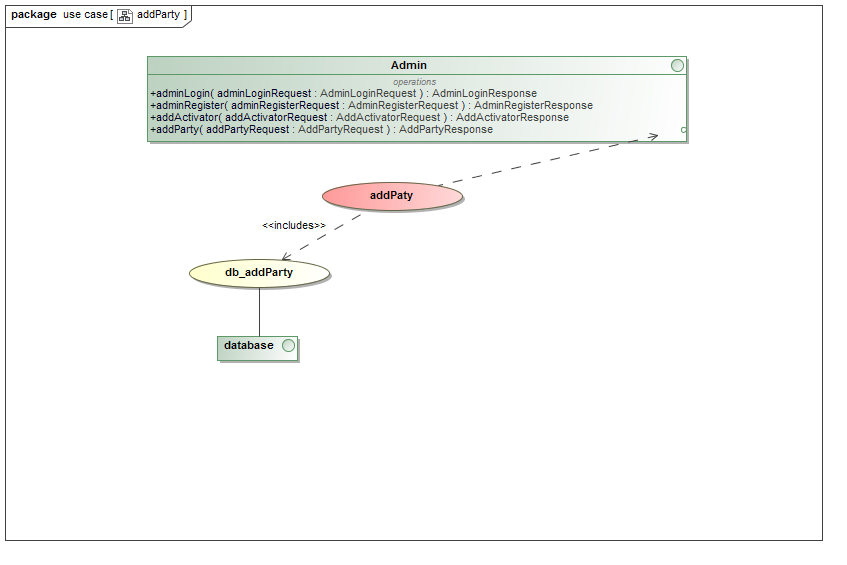
\includegraphics[width=0.75\linewidth]{../Images/Admin/UseCases/addParty_useCase.png}
				\caption{Add Party Use Case}
			\end{figure}
			
			The addVoter function will call the validateData function, and if the data is valid, it will call the Database addPoliticalParty function.
			\newline
			
			\item \textbf{Process Design}
			\begin{figure}[H]
				\centering
				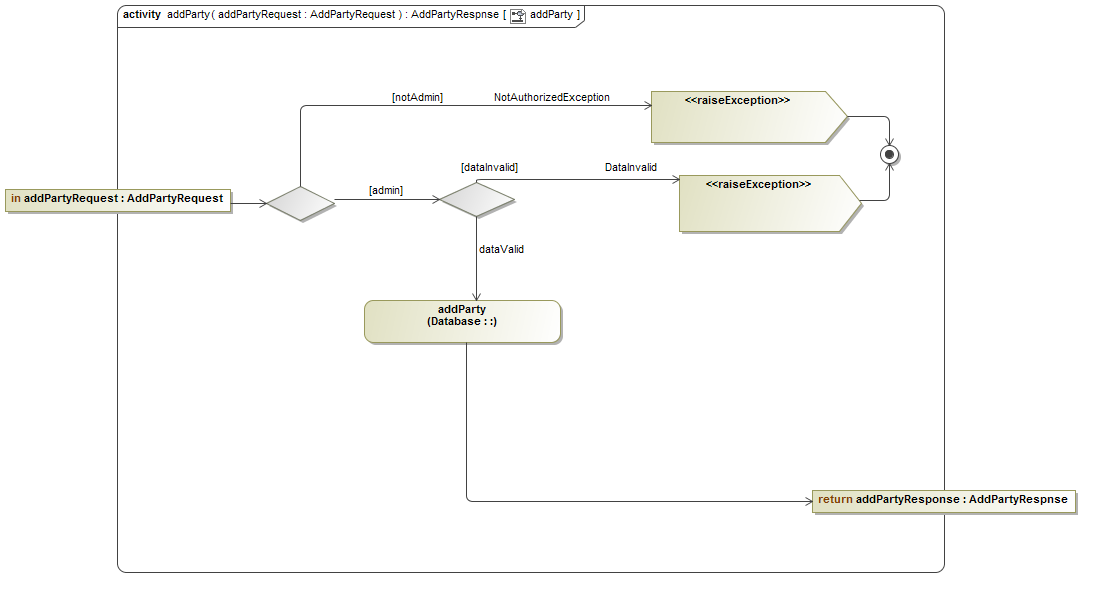
\includegraphics[width=0.75\linewidth]{../Images/Admin/ActivityDiagrams/addParty_ActivityDiagram.png}
				\caption{Add Party Activity}
			\end{figure}
			
		The addParty function will first check that a database connection exists and throw an appropriate exception otherwise. Once it has established a connection, it will then check to see if the new party the Admin wants to add does not already exist in the database. If the party already exists, an appropriate exception is thrown. If the party does not exist, the new party data is validated - with an exception being thrown if it is not valid, but if it is valid, then the new party data is successfully persisted to the database. 
			\newline
			
		\end{enumerate}
\end{enumerate}